\documentclass{standalone}
\usepackage{tikz}
\usepackage[colorlinks=true]{hyperref}
\usetikzlibrary{
  arrows,
  calc,
  decorations.pathmorphing,
  decorations.pathreplacing,
  decorations.markings,
  positioning,
  shapes,
  arrows.meta
}

\ifpdf
% Ensure reproducible output
\pdfinfoomitdate=1
\pdfsuppressptexinfo=-1
\pdftrailerid{}
\hypersetup{
  pdfcreator={},
  pdfproducer={}
}
\fi

\begin{document}

\begin{tikzpicture}
  \begin{scope}[rotate=-90]
    \clip(-2.5,-0.85) rectangle (2.5, 0.85);
    \begin{scope}
      \clip plot[samples=200,domain=-2.5:2.5] function {sqrt(0.005 + x**2 / 4)}
      -- plot[samples=200,domain=2.5:-2.5] function {-sqrt(0.005 + x**2 / 4)};
      \node[rotate=90] at (0, 0)
      {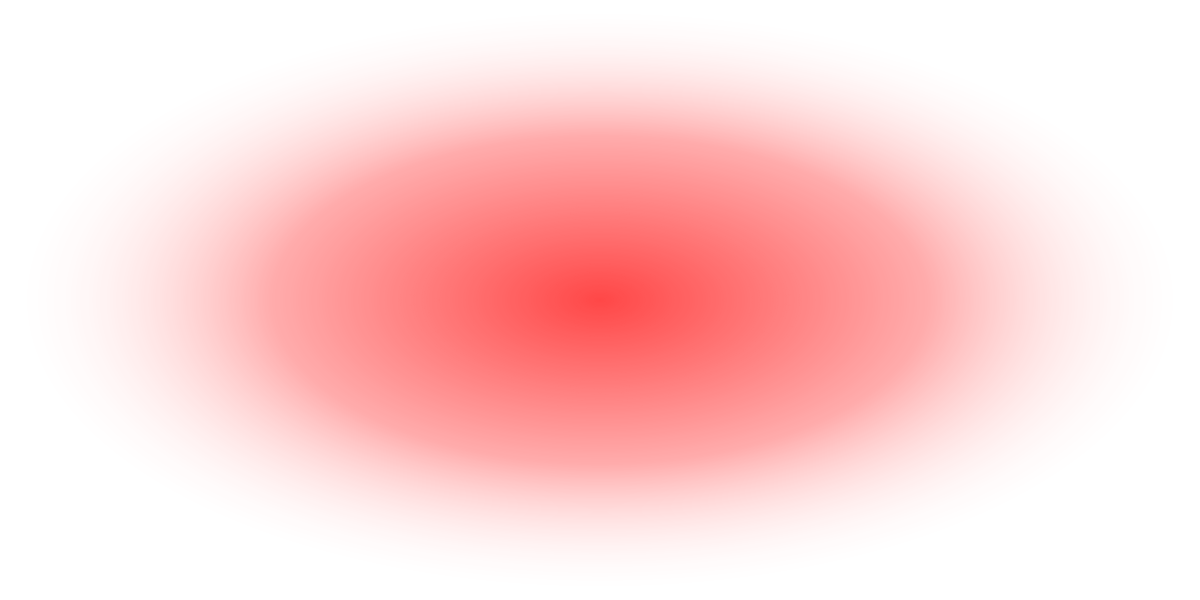
\includegraphics[width=5cm,height=2.504cm]{fadings/red_tweezer.png}};
      \fill[white] plot[draw,samples=200,domain=1.2:2.5] function {sqrt(0.005 + x**2 / 4)}
      -- plot[draw,samples=200,domain=2.5:1.2] function {-sqrt(0.005 + x**2 / 4)};
    \end{scope}
  \end{scope}
  \draw[black,fill=white,line width=1] (0.605, -1.2) -- (0.85, -1.6) -- (0.85, -3.2) --
  (-0.85, -3.2) -- (-0.85, -1.6) -- (-0.605, -1.2) -- cycle;
  \node[below] at (0, -3.2) {\large Objective};

  \draw[<->,>=stealth,line width=0.7,red!50!black] (0.3, 0) -- (-0.3, 0)
  node[right,align=center] at (0.3, -0.2) {\large Raman \&\\\large Tweezer};

  \draw[->,>=stealth,line width=0.7] (-0.5, 0.2) -- node[below] {\large $B_0$} (-1.05, 0.2);
\end{tikzpicture}

\end{document}
